\documentclass[notes,11pt, aspectratio=169, xcolor=table]{beamer}

\usepackage{pgfpages}
% These slides also contain speaker notes. You can print just the slides,
% just the notes, or both, depending on the setting below. Comment out the want
% you want.
\setbeameroption{hide notes} % Only slide
%\setbeameroption{show only notes} % Only notes
%\setbeameroption{show notes on second screen=right} % Both

\usepackage{helvet}
\usepackage[default]{lato}
\usepackage{array}
\usepackage{minted}

\newtheorem{proposition}{Proposition}

\usepackage{tikz}
\usetikzlibrary{shapes.geometric}
\usepackage{pgfplots}
\usepackage{graphicx}
\usepackage{verbatim}
\setbeamertemplate{note page}{\pagecolor{yellow!5}\insertnote}
\usetikzlibrary{positioning}
\usetikzlibrary{snakes}
\usetikzlibrary{calc}
\usetikzlibrary{arrows}
\usetikzlibrary{decorations.markings}
\usetikzlibrary{shapes.misc}
\usetikzlibrary{matrix,shapes,arrows,fit,tikzmark}
\usepackage{amsmath}
\usepackage{mathpazo}
\usepackage{hyperref}
\usepackage{lipsum}
\usepackage{multimedia}
\usepackage{graphicx}
\usepackage{multirow}
\usepackage{graphicx}
\usepackage{dcolumn}
\usepackage{bbm}
\usepackage[style=authoryear,sorting=nyt,uniquename=false]{biblatex}

\addbibresource{references.bib} 

\newcolumntype{d}[0]{D{.}{.}{5}}

\def\@@mybluebox[#1][#2]#3{
    \sbox\mytempbox{#3}%
    \mytemplen\ht\mytempbox
    \advance\mytemplen #1\relax
    \ht\mytempbox\mytemplen
    \mytemplen\dp\mytempbox
    \advance\mytemplen #2\relax
    \dp\mytempbox\mytemplen
    \colorbox{myblue}{\hspace{1em}\usebox{\mytempbox}\hspace{1em}}}


\usepackage{changepage}
\usepackage{appendixnumberbeamer}
\newcommand{\beginbackup}{
   \newcounter{framenumbervorappendix}
   \setcounter{framenumbervorappendix}{\value{framenumber}}
   \setbeamertemplate{footline}
   {
     \leavevmode%
     \hline
     box{%
       \begin{beamercolorbox}[wd=\paperwidth,ht=2.25ex,dp=1ex,right]{footlinecolor}%
%         \insertframenumber  \hspace*{2ex} 
       \end{beamercolorbox}}%
     \vskip0pt%
   }
 }
\newcommand{\backupend}{
   \addtocounter{framenumbervorappendix}{-\value{framenumber}}
   \addtocounter{framenumber}{\value{framenumbervorappendix}} 
}


\usepackage{graphicx}
\usepackage[space]{grffile}
\usepackage{booktabs}

% These are my colors -- there are many like them, but these ones are mine.
\definecolor{blue}{RGB}{0,114,178}
\definecolor{red}{RGB}{213,94,0}
\definecolor{yellow}{RGB}{240,228,66}
\definecolor{green}{RGB}{0,158,115}

\hypersetup{
  colorlinks=false,
  linkbordercolor = {white},
  linkcolor = {blue}
}


%% I use a beige off white for my background
\definecolor{MyBackground}{RGB}{255,253,218}

%% Uncomment this if you want to change the background color to something else
%\setbeamercolor{background canvas}{bg=MyBackground}

%% Change the bg color to adjust your transition slide background color!
\newenvironment{transitionframe}{
  \setbeamercolor{background canvas}{bg=yellow}
  \begin{frame}}{
    \end{frame}
}

\setbeamercolor{frametitle}{fg=blue}
\setbeamercolor{title}{fg=blue}
\setbeamertemplate{footline}[frame number]
\setbeamertemplate{navigation symbols}{} 
\setbeamertemplate{itemize items}{-}
\setbeamercolor{itemize item}{fg=blue}
\setbeamercolor{itemize subitem}{fg=blue}
\setbeamercolor{enumerate item}{fg=blue}
\setbeamercolor{enumerate subitem}{fg=blue}
\setbeamercolor{button}{bg=MyBackground,fg=blue,}



% If you like road maps, rather than having clutter at the top, have a roadmap show up at the end of each section 
% (and after your introduction)
% Uncomment this is if you want the roadmap!
% \AtBeginSection[]
% {
%    \begin{frame}
%        \frametitle{Roadmap of Talk}
%        \tableofcontents[currentsection]
%    \end{frame}
% }
\setbeamercolor{section in toc}{fg=blue}
\setbeamercolor{subsection in toc}{fg=red}
\setbeamersize{text margin left=1em,text margin right=1em} 

\newenvironment{wideitemize}{\itemize\addtolength{\itemsep}{10pt}}{\enditemize}

\usepackage{environ}
\NewEnviron{videoframe}[1]{
  \begin{frame}
    \vspace{-8pt}
    \begin{columns}[onlytextwidth, T] % align columns
      \begin{column}{.58\textwidth}
        \begin{minipage}[t][\textheight][t]
          {\dimexpr\textwidth}
          \vspace{8pt}
          \hspace{4pt} {\Large \sc \textcolor{blue}{#1}}
          \vspace{8pt}
          
          \BODY
        \end{minipage}
      \end{column}%
      \hfill%
      \begin{column}{.42\textwidth}
        \colorbox{green!20}{\begin{minipage}[t][1.2\textheight][t]
            {\dimexpr\textwidth}
            Face goes here
          \end{minipage}}
      \end{column}%
    \end{columns}
  \end{frame}
}

\title[]{International Trade: Data Lab 3}
\subtitle[]{Your first numerical model}
\author[Góes]
{Carlos Góes\inst{1}}
\date{Fall 2025}
\institute[GWU]{\inst{1} George Washington University }



\begin{document}

%%% TIKZ STUFF
\tikzset{   
        every picture/.style={remember picture,baseline},
        every node/.style={anchor=base,align=center,outer sep=1.5pt},
        every path/.style={thick},
        }
\newcommand\marktopleft[1]{%
    \tikz[overlay,remember picture] 
        \node (marker-#1-a) at (-.3em,.3em) {};%
}
\newcommand\markbottomright[2]{%
    \tikz[overlay,remember picture] 
        \node (marker-#1-b) at (0em,0em) {};%
}
\tikzstyle{every picture}+=[remember picture] 
\tikzstyle{mybox} =[draw=black, very thick, rectangle, inner sep=10pt, inner ysep=20pt]
\tikzstyle{fancytitle} =[draw=black,fill=red, text=white]
%%%% END TIKZ STUFF



%----------------------------------------------------------------------%
%-------------------       TITLE PAGE       ---------------------------%
%----------------------------------------------------------------------%





%----------------------------------------------------------------------%






%----------------------------------------------------------------------%
%----------------------------------------------------------------------%

%----------------------------------------------------------------------%
\frame{\titlepage}
\addtocounter{framenumber}{-1}
%----------------------------------------------------------------------%



%----------------------------------------------------------------------%
%----------------------------------------------------------------------%

\section{Introduction}

\begin{frame}{Plan for today}

\begin{wideitemize}
    \item Introduce custom-made functions in Python
    \item Write down functions that map our model to the computer
    \item Input values for parameters
    \item Understand the logic of solving the model
    \item Try to solve it Python
\end{wideitemize}
    
\end{frame}


\begin{frame}{Labor Market Equilibrium}
    \begin{wideitemize}
        \item Combining the three equations above:

    { \scriptsize
    \begin{equation*}
        P_{M} \times  Z_{i,M} \times (1-\beta_i) \times \left( \frac{K_{i}}{L_{i,M}} \right)^{\beta_i} = P_{A} \times  Z_{i,A} \times (1-\beta_i) \times \left( \frac{T_{i}}{\bar{L}_i - L_{i,M}} \right)^{\beta_i} 
    \end{equation*}
    }
    \item<2-> Rearrange terms: 

        { \scriptsize
    \begin{equation*}
        \frac{P_{M} \times  Z_{i,M}}{P_{A} \times  Z_{i,A}} \times \left( \frac{K_{i}}{T_{i}} \right)^{\beta_i} \times (\bar{L}_i - L_{i,M})^{\beta_i} =  L_{i,M}^{\beta_i} 
    \end{equation*}
    }

    \item<3-> Raise both sides to $\beta_i$:

            { \scriptsize
    \begin{equation*}
         \left( \frac{P_{M} \times  Z_{i,M}}{P_{A} \times  Z_{i,A}} \right)^{\frac{1}{\beta_i}} \times  \frac{K_{i}}{T_{i}} \times (\bar{L}_i - L_{i,M}) =  L_{i,M} 
    \end{equation*}
    }    

    \item<4-> Define $\Omega_i = \left( \frac{P_{M} \times  Z_{i,M}}{P_{A} \times  Z_{i,A}} \right)^{\frac{1}{\beta_i}} \times  \frac{K_{i}}{T_{i}}$.


    \end{wideitemize}
\end{frame}


\begin{frame}{Labor Market Equilibrium}
    \begin{wideitemize}
        \item What is $\Omega_i = \left( \frac{P_{M} \times  Z_{i,M}}{P_{A} \times  Z_{i,A}} \right)^{\frac{1}{\beta_i}} \times  \frac{K_{i}}{T_{i}}$? This term reflects: 
        \begin{itemize}
            \item relative profitability and tech, scaled by how responsive production is to labor (via $\beta_i$); and
            \item relative capacity of the two sectors to employ labor, given the specific factors ($K_i$, $T_i$).
        \end{itemize}
        \item<2-> Then:
        \begin{equation*}
         \Omega_i \times (\bar{L}_i - L_{i,M}) =  L_{i,M} \iff  L_{i,M} = \frac{\Omega_i}{1+\Omega_i} \times \bar{L}_i
         \end{equation*}
         \item<3-> ...and:
        \begin{equation*}
           L_{i,A} = \bar{L}_i - L_{i,M} =  \frac{1}{1+\Omega_i}  \times  \bar{L}_i
        \end{equation*}

        \item<4-> Note: $L_{i,M} / L_{i,A} = \Omega_i$
        \qquad (parameters in $\Omega_i$ pin down relative labor allocation) 
        
    \end{wideitemize}
\end{frame}

\begin{frame}[fragile=singleslide]{From theory to computing}

\begin{wideitemize}
    \item First let us define the parameters:

        \begin{minted}{python}
            Z_M = {'H':1.0, 'F':1.0} 
            Z_A = {'H':1.0, 'F':1.0} 
            K   = {'H':4.0, 'F':2.0} 
            T   = {'H':3.0, 'F':1.0} 
            L   = {'H':5.0, 'F':5.0}
            beta= {'H':0.40,'F':0.40}
            alpha={'H':0.50,'F':0.50}
        \end{minted}    

    
    \item Let $\frac{P_{M}}{P_{A}}\equiv p$, the relative price. Then we can write omega as a function of $i,p$:

    \begin{equation*}
        \Omega(i,p) = \left( p \times\frac{Z_{i,M}}{Z_{i,A}} \right)^{\frac{1}{\beta_i}} \times  \frac{K_{i}}{T_{i}}
    \end{equation*}

    \item In the computer:

        \begin{minted}{python}
        def Omega(i, p):
            return (p * Z_M[i]/Z_A[i])**(1.0/beta[i]) * (K[i]/T[i])
        \end{minted}    

\end{wideitemize}
    
\end{frame}


\begin{frame}[fragile=singleslide]{Labor allocations}

        \begin{equation*}
         L_{M}(i,p) = \frac{\Omega(i,p)}{1+\Omega(i,p)} \times \bar{L}_i
         \end{equation*}

        \begin{minted}{python}
            def Lm(i, p):
                return (Omega(i, p)/(1+Omega(i, p))) * L[i]
        \end{minted}    

        \begin{equation*}
           L_{A}(i,p) = \bar{L}_i - L_{M}(i,p) =  \frac{1}{1+\Omega(i,p)}  \times  \bar{L}_i
        \end{equation*}

        \begin{minted}{python}
            def La(i, p):
                return L[i] - Lm(i, p)
        \end{minted}    


\end{frame}

\begin{frame}[fragile=singleslide]{Production}

\begin{itemize}
    \item Production with sector-specific factors land \blue{$T$} and capital \blue{$K$}:
        \begin{eqnarray*}\label{eq: production}
            Y_{M}(i,p) &=&  Z_{i,M} \times K_{i}^{\beta_i} [L_{M}(i,p)]^{1-\beta_i}  \\
            Y_{A}(i,p) &=&  Z_{i,A} \times T_{i}^{\beta_i} [L_{A}(i,p)]^{1-\beta_i} 
        \end{eqnarray*}

        \begin{minted}{python}
            def Ym(i, p):
                return Z_M[i]*K[i]**beta[i] * Lm(i,p)**(1-beta[i])

            def Ya(i, p):
                return Z_A[i]*T[i]**beta[i] * La(i,p)**(1-beta[i])
        \end{minted}
\end{itemize}
    
\end{frame}


\begin{frame}[fragile=singleslide]{Relative Supply}

\begin{wideitemize}
    
    \item Relative supply:

    \begin{equation*}
        RS(p) = \frac{Y_{M}(H,p) + Y_{M}(F,p)}{Y_{A}(H,p) + Y_{A}(F,p)}
    \end{equation*}

    note that this sums over $\{ H, F \}$. Does not depend on $i$.
        \begin{minted}{python}
        def RS(p):
            num = sum(Ym(i,p) for i in ['H','F'])
            den = sum(Ya(i,p) for i in ['H','F'])
            return num/den    
        \end{minted}
        
    
\end{wideitemize}

    
\end{frame}


\begin{frame}[fragile=singleslide]{Total income}

\begin{wideitemize}
    
    \item Total value of production is distributed to HH either as rents or income (why?)

    \begin{equation*}
        I(i,p) = p Y_M(i,p) + Y_A(i,p)
    \end{equation*}

    \begin{minted}{python}
        def I(i,p):
            return p*Ym(i,p) + Ya(i,p)
    \end{minted}

    
\end{wideitemize}

    
\end{frame}


\begin{frame}[fragile=singleslide]{Demand}

\begin{wideitemize}
    
    \item  Cobb-Douglas: demand = constant share of income; decreasing in price:
    \begin{equation*}\label{eq: demand}
    Q_{i,A} = \alpha_i  \frac{I_i}{P_{A}} , \qquad Q_{i,M} = (1-\alpha_i) \frac{I_i}{P_{M}}
    \end{equation*}

    \item Since we are solving for relative prices $p = P_M/P_A$, this is like setting $P_A =1.0$:

    \begin{equation*}
    Q_{A}(i,p) = \alpha_i  I(i,p)  , \qquad Q_{M}(i,p) = (1-\alpha_i) \frac{I(i,p)}{p}
    \end{equation*}

    \begin{minted}{python}
    def Qa(i, p):
        return (alpha[i])*I(i,p)

    def Qm(i, p):
        return (1-alpha[i])*I(i,p)/p
    \end{minted}

        
    
\end{wideitemize}

    
\end{frame}

\begin{frame}[fragile=singleslide]{Relative demand}

    \begin{equation*}
        RD(p) = \frac{Q_{M}(H,p) + Q_{M}(F,p)}{Q_{A}(H,p) + Q_{A}(F,p)}
    \end{equation*}

    note that this sums over $\{ H, F \}$. Does not depend on $i$. \\
    
        \begin{minted}{python}
        def RD(p):
            num = sum(Qm(i,p) for i in ['H','F'])
            den = sum(Qa(i,p) for i in ['H','F'])
            return num/den
        \end{minted}

\end{frame}


\begin{frame}{Trade Equilibrium: Global Demand and Supply}
\begin{figure}
    \centering
        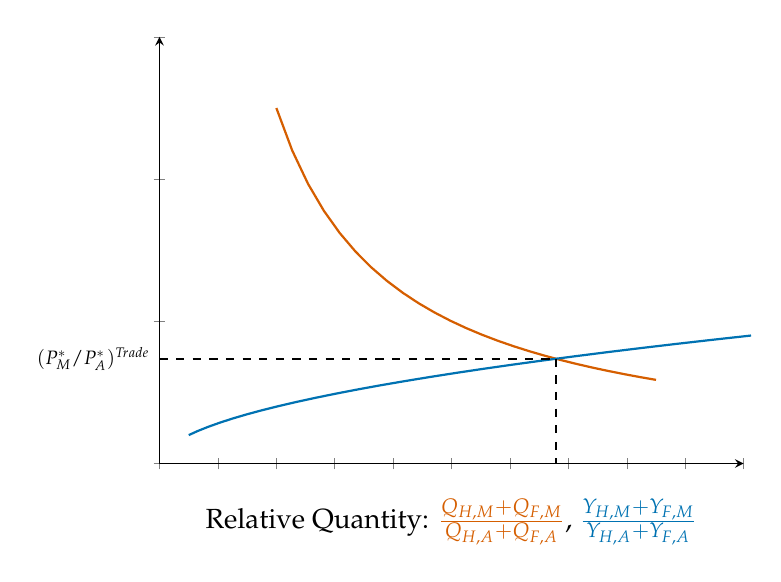
\begin{tikzpicture}
        
    \pgfmathsetmacro{\beta}{1/3}
    \pgfmathsetmacro{\alpha}{0.5}

    \pgfmathsetmacro{\Zm}{1}
    \pgfmathsetmacro{\K}{4}
    
    \pgfmathsetmacro{\Za}{1}
    \pgfmathsetmacro{\T}{1}

    \pgfmathsetmacro{\Kf}{1}
    \pgfmathsetmacro{\Tf}{1}


    \pgfmathsetmacro{\Ps}{\Za/\Zm * ((1-\alpha)/\alpha * \T / \K)^(\beta)}   
    \pgfmathsetmacro{\Qs}{(1-\alpha)/\alpha / \Ps}

    \pgfmathsetmacro{\Psf}{\Za/\Zm * ((1-\alpha)/\alpha * \Tf / \Kf)^(\beta)}   
    \pgfmathsetmacro{\Qsf}{(1-\alpha)/\alpha / \Psf}

    \pgfmathsetmacro{\Psw}{\Za/\Zm * ((1-\alpha)/\alpha * ( ( \T + \Tf) / (\K+\Kf ) )^(\beta)}   
    \pgfmathsetmacro{\Qsw}{(1-\alpha)/\alpha / \Psw}

    
    

        \centering
        \begin{axis}[
            xlabel={Relative Quantity: \textcolor{red}{$\frac{Q_{H,M} + Q_{F,M}}{Q_{H,A} + Q_{F,A}}$}, \textcolor{blue}{$\frac{Y_{H,M} + Y_{F,M}}{Y_{H,A} + Y_{F,A}}$}},
            ymin=0, ymax=3,
            xmin=0, xmax=2,
            yticklabel=\empty,
            xticklabel=\empty,
            axis lines=left,
            enlargelimits=false,
            clip=false,
            axis on top,
            scaled x ticks=false,
            width=9cm, height=7cm,
            title style={font=\bfseries}
        ]
        
        % demand
        \addplot[domain=0.4:1.7, thick, red] (x, {(1-\alpha)/\alpha / x});
        % supply world
        \addplot[domain=0.2:0.9, thick, blue] ({(\Zm/\Za)^(1/\beta) * ( (\K+\Kf) / (\T+\Tf) ) * x^((1-\beta)/\beta)}, x);
        %\addplot[domain=0.2:1.3, thick, blue] (x, {(\Zm/\Za)^(- 1/\beta) * x^((1-\beta)/\beta) * ( (\Kf + \K) / ( \Tf + \T ) ) });
        
        \addplot[dashed, thick] coordinates {(0,\Psw) (\Qsw,\Psw)};
        \node[black, anchor=east] at (axis cs:0,\Psw) {\scriptsize $(P_{M}^*/P_{A}^*)^{Trade}$};
        \addplot[dashed, thick] coordinates {(\Qsw,\Psw) (\Qsw,0)};

        %\addplot[dashed] coordinates {(0,\Psw) (\Qsw,\Psw)};
        %\node[black] at (axis cs:-0.1,\Psw) {\small $(P_{M}^*/P_{A}^*)^{Trade}$};
        %\addplot[dashed] coordinates {(\Qsw,\Psw) (\Qsw,0)};
        % \node[black] at (axis cs:\Qs,-0.15) {\small $\textcolor{red}{RD_i} = \textcolor{blue}{RS_i}$};

        
        %\addplot[thick, dashed, domain=0:5] {0.5};
        
        \end{axis}
        
        \end{tikzpicture}
        \caption{World Trade Equilibrium}
    \label{fig: trade-eqm}
\end{figure}
\end{frame}

\begin{frame}{How to solve for prices?}

\begin{wideitemize}
    \item Define excess demand function:

    \begin{equation*}
        ED(p) = RS(p) - RD(p)
    \end{equation*}

    \item This should be strictly increasing in price (check the figure above) -- it only crosses zero once

    \item Equilibrium price $p^*$ defined as the price for which supply equals demand:

    \begin{equation*}
        ED(p^*) = 0 \iff RS(p^*) = RD(p^*)
    \end{equation*}
    
\end{wideitemize}


    
\end{frame}



\begin{frame}{Excess Demand Function}
\begin{figure}
    \centering
    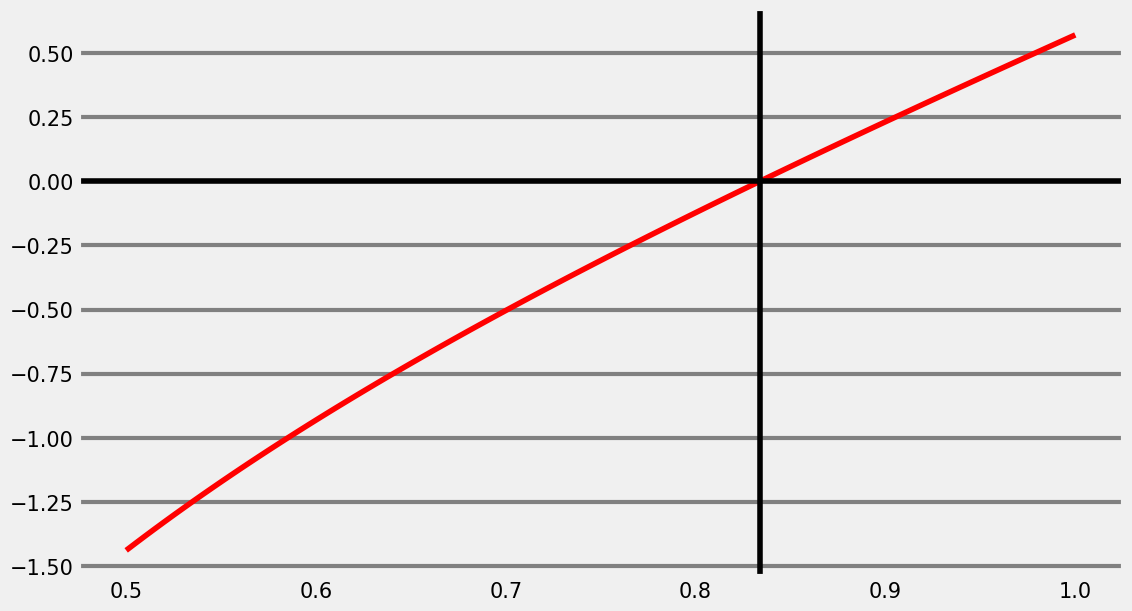
\includegraphics[width=0.75\linewidth]{figs/ed.png}
    \caption{Excess Demand Function}
    \label{fig:ed}
\end{figure}
\end{frame}

\begin{frame}{Bisection Method}
\begin{figure}
    \centering
    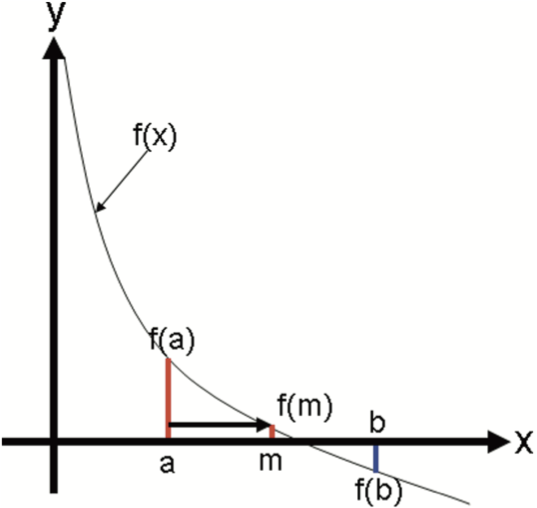
\includegraphics[width=0.5\linewidth]{figs/bisection-method.png}
    \caption{Root finding with bi-section method}
    \label{fig:ed}
\end{figure}
\end{frame}

\begin{frame}{Logic of algorithm}

\begin{wideitemize}
    \item Choose some small tolerance level $\varepsilon>0$ 
    
    \item Pick $a$, such that $ED(a) <0$ and $b$ such that $ED(b)>0$

    \item Calculate the median point $m = 1/2(a+b)$

    \item Calculate $ED(m)$

    \item If $ED(m)$ is positive ($ED(m)\times ED(a) <0$): update $b=m$

    \item If $ED(m)$ is negative ($ED(m)\times ED(a) \ge 0$): update $a=m$

    \item Repeat until $f(m) < \epsilon$

\end{wideitemize}
    
\end{frame}

\begin{frame}[fragile=singleslide]{Algorithm}

\begin{minted}{python}
    def bisect_root(f, a, b, tol=1e-6, max_iter=100):
    fa, fb = f(a), f(b)
    if fa*fb > 0:
        raise ValueError("Root not bracketed: f(a),f(b) same sign")
    for iter in range(max_iter):
        m = 0.5*(a+b)
        fm = f(m)
        if abs(fm) < tol or (b-a)<tol:
            return m
        if fa*fm < 0:
            b, fb = m, fm
        else:
            a, fa = m, fm
    raise RuntimeError("Bisection failed to converge")
\end{minted}

\end{frame}

\begin{frame}[fragile=singleslide]{Solve for prices}
    \begin{minted}{python}
p_low, p_high = 1, 1
# shrink/expand until signs differ
while excess_demand(p_low) > 0:
    p_low = p_low/2
while excess_demand(p_high) < 0:
    p_high = p_high*2

p_star = bisect_root(excess_demand, p_low, p_high)  
print("Equilibrium P_M/P_A =", p_star)
[1] Equilibrium P_M/P_A = 0.833808422088623
    \end{minted}
\end{frame}

\end{document}



                xlabel={Relative Quantity: \textcolor{red}{$\frac{Q_{H,M} + Q_{F,M}}{Q_{H,A} + Q_{F,A}}$}, \textcolor{blue}{}},
